\documentclass[../main]{subfiles}
\begin{document}

\chapter{Private key encryption}

\section{Asymptotic approach}

\begin{definition}[PPT Algorithm]
    A probabilistic algorithm $A$ is said to be \textbf{Probabilistic Polynomial Time (PPT)} if there is a polynomial $p$ that defines an upper bound on the computation time
    of $A$ independently of the probabilistic choices made by the latter.
\end{definition}

\begin{definition}[Negligible function]
    A function $f: \mathbb{N} \rightarrow{} \mathbb{R}$ is said to be \textit{negligible} if and only if for every polynomial $p: \mathbb{N} \rightarrow{} \mathbb{N}$
    there exists $N \in{} \mathbb{N}$ such that for every $n > N$ it holds that $f(n) < \frac{1}{p(n)}$.
\end{definition}

\begin{lemma}[Closure of the set of negligible functions]
    \label{lemma:closure-ngl-functions}
    The set of all negligible functions, called $\mathcal{NGL}$, is closed for sum, product, and product by an arbitrary polynomial.
\end{lemma}

\paragraph{Proof}
Suppose $\epsilon$ is a negligible function. Let $p: \mathbb{N} \rightarrow{} \mathbb{N}$ be any polynomial.\\
We want to prove that:
$$\epsilon'(n) = \epsilon(n)\cdot{}p(n)$$
is itself negligible.\\
We know that $\forall{} q: \mathbb{N} \rightarrow{} \mathbb{N}$ $\exists{} N \in{} \mathbb{N}\; s.t.\;\forall{} n > N$
$$\epsilon(n) < \frac{1}{p(n)\cdot{}q(n)}$$
Let us prove that $\epsilon'(n)$ is negligible, namely that $\forall{} q: \mathbb{N} \rightarrow{} \mathbb{N}$ $\exists{} N \in{} \mathbb{N}\; s.t.\;\forall{} n > N$
$$\epsilon'(n) < \frac{1}{q(n)}$$
To conclude, we know that:
$$\epsilon'(n) = \epsilon(n) \cdot{} p(n) < \frac{1}{q(n)\cdot{}p(n)} \cdot{} p(n)$$
and therefore \ref{lemma:closure-ngl-functions} is proved.

\section{Proofs by reduction}

In the context of computational cryptography we have $|\mathcal{K}| \ll{} |\mathcal{M}|$ hence the adversary could construct ``easily'' two attacks:
\begin{itemize}
    \item (ciphertext-only) given a ciphertext $c$ the attacker could try to decrypt $c$ \textbf{with all possible keys} (it is a brute-force attack, of course, but perhaps feasible);
    \item (known-plaintext) given couples ($m_1$, $c_1$), ..., ($m_l$, $c_l$) the attacker could try to generate a key $k$ randomly and then check whether $Dec_k(c_i) = m_i$ for every $i$.
\end{itemize}
The probability of success of the attacker must be minimized, together with its computational power.
We would have to prove the following:
$$\forall{} A \in{} PPT \; \neg BRK(\Pi, A) \Leftrightarrow{} \nexists{} A \in{} PPT \; \neg BRK(\Pi, A)$$
in which $BRK(\Pi, A)$ means ``Algorithm/attacker A breaks scheme $\Pi$'', but that is currently impossible to prove.\\
The only thing we can prove right now is the following:
$$\forall{} B \in{} PPT \; \neg BRK(\Xi, B) \Rightarrow{} \forall{} A \in{} PPT \; \neg BRK(\Pi, A)$$
$$\Updownarrow$$
$$\exists{} A \in{} PPT \; BRK(\Pi, A) \Rightarrow{} \exists{} B \in{} PPT \; BRK(\Xi, B)$$
\begin{figure}[h]
    \centering
    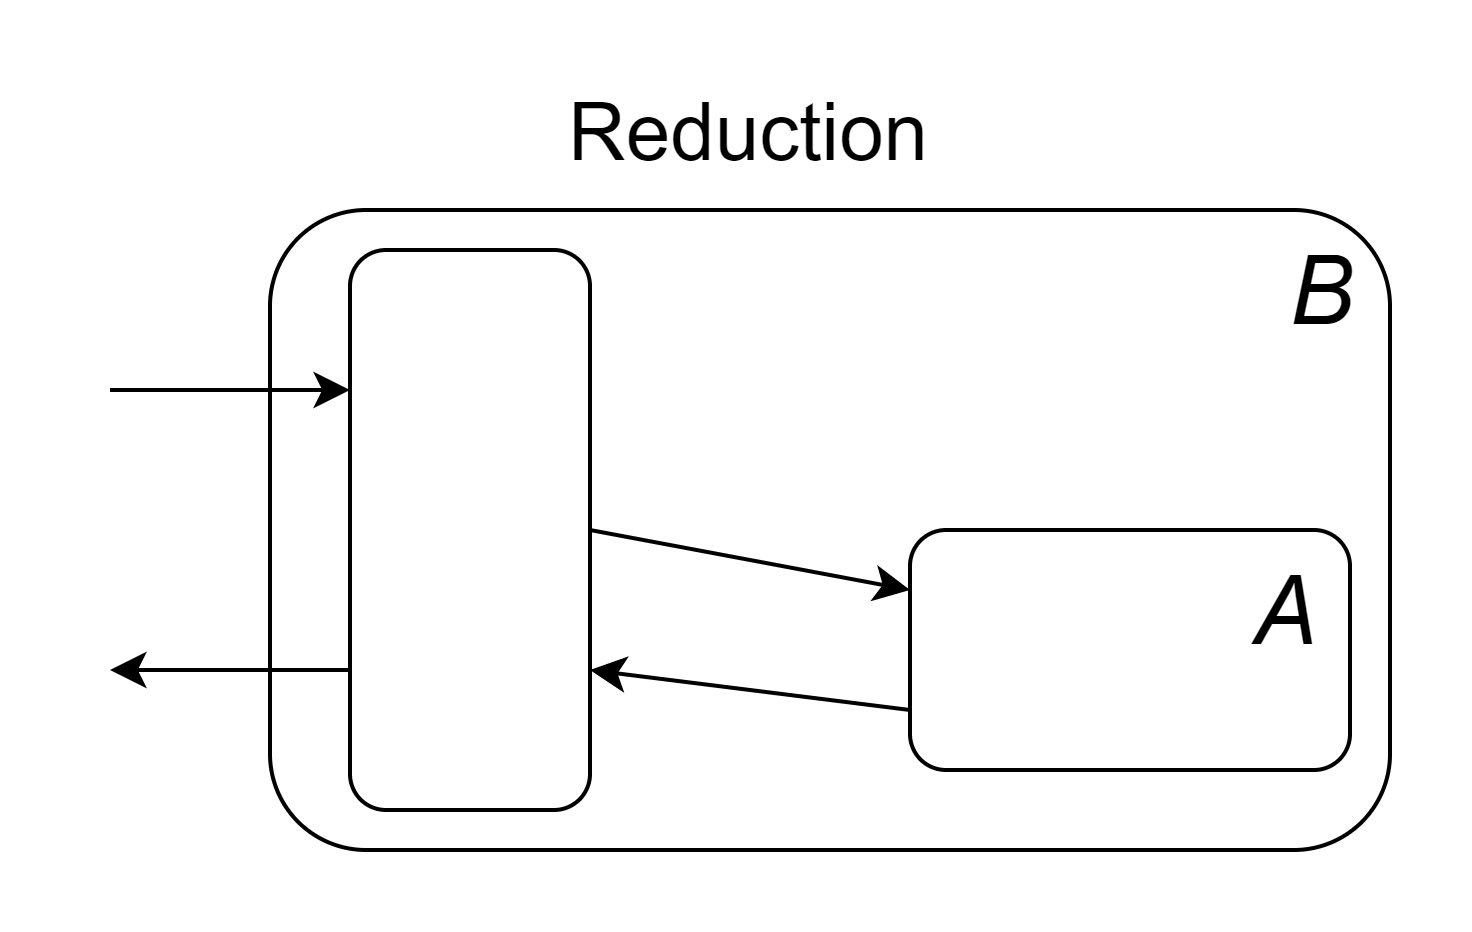
\includegraphics[width=0.5\textwidth]{images/reduction}
    \caption{Graphical representation of proofs by reduction.}
\end{figure}
\paragraph{Proof (by means of contradiction)}
Assuming that $\Xi$ is not solvable by efficient (PPT) algorithms, a part from those with negligible probability, we want therefore to prove that $\Pi$ is secure ($\forall{} B \in{} PPT \; \neg BRK(\Xi, B) \Rightarrow{} \forall{} A \in{} PPT \; \neg BRK(\Pi, A)$).\\
\begin{enumerate}
    \item Let's say that it exists $A \in PPT$, an efficient algorithm for solving $\Pi$ and that the probability of solving it is $\epsilon(n)$ (which is a polynomial function).
    \item Now let's take $B \in{} PPT$, which is an efficient algorithm for solving $\Xi$, that uses $A$ as a subroutine internally without knowing how it works.
    It just knows how the inputs map to outputs. Given an instance $\xi$ of $\Xi$, $B$ simulates $\Pi$ for $A$; $A$ must not see any difference (inputs and outputs given to $A$ should respect the pre- and post-conditions of $\Pi$).
    If $A$ breaks $\Pi$ then $B$ should be able to solve $\Xi$ with instance $\xi$ with probability \textbf{at least} $\frac{1}{p(n)}$ (inverse polynomial).
    \item If $\epsilon(n)$ is not negligible (which is not, because of assumptions made in step 1), then $B$ solves $\Xi$ with probability $\frac{\epsilon(n)}{p(n)}$ which is not negligible (hence polynomial/efficient).
    Since $B$ is efficient, and we know that $A$ is efficient too, we showed that $B$ can solve $\Xi$ with non-negligible probability. Which is impossible because it violates the initial assumptions.
    \item To conclude, given the assumption on $\Xi$, no efficient algorithm $A$ can solve $\Pi$ with non-negligible probability $\epsilon(n)$ and $\Pi$ is computationally secure. 
\end{enumerate}

\section{New definition of encryption scheme}
An encryption scheme in computational cryptography has the form $\Pi{} = (Gen, Enc, Dec)$ with $Gen, Enc, Dec \in{} PPT$ and:
\begin{itemize}
    \item $k \leftarrow{} Gen(1^n) \; s.t. \; |k| \ge{} n$. The parameter $n$ is regarded as the \textbf{security parameter};
    \item $Enc$ is probabilistic and therefore $Enc(m, k)$ can output different ciphertexts every time with the same couple $(m, k)$. Note that $k$ has no information on $n$ but it has been generated from it;
    \item $Dec$ is by the way purely deterministic, otherwise there would not be any way to get the original message $m$ from a given $c$;
    \item The scheme is correct: $Dec_k(Enc_k(m)) = m$;
    \item $Enc_k(m)$ can work with messages of length $l(n)$, where $n$ is the security parameter and $l$ is a function on it. For example, the OTP would have $l(n) = n$ (the identity function).
\end{itemize}
We need to update the experiment for understanding whether the scheme is secure:\\
$PrivK^{eav}_{A,\Pi}(n)$:\\
$(m_0,m_1) \; \leftarrow{} \; A(1^n)$\\
\textbf{if} $|m_0| \; \neq{} \; |m_1|$ \textbf{then}\\
\hspace*{20pt}\textbf{Result}: 0\\
$k \; \leftarrow{} \; Gen(1^n)$\\
$b \; \leftarrow{} \; \{0,1\}$\\
$c \; \leftarrow{} \; Enc(k,m_b)$\\
$b^* \; A(c)$\\
\textbf{Result}: $\neg(b \oplus{} b^*)$
\begin{definition}[Security of an encryption scheme]
    An encryption scheme $\Pi$ is said to be \textit{secure against passive attacks} (i.e., when the attacker does not know the $Enc$ and $Dec$ functions) or \textit{secure w.r.t.} $PrivK^{eav}$
    if and only if for each PPT adversary $A$ there exists a function $\epsilon{} \in{} \mathcal{NGL}$ s.t.
    $$Pr(PrivK^{eav}_{A,\Pi}(n) = 1) = \frac{1}{2} + \epsilon(n)$$
\end{definition}
As a note, $\frac{1}{2}$ corresponds to the probability we required also in the previous experiment. We are now adding only a negligible probability $\epsilon(n)$.

\section{Pseudo randomness}
Since we cannot require anymore that $|\mathcal{M}| = |\mathcal{K}|$ and only that $|\mathcal{K}| < |\mathcal{M}|$ we must find a way to make the generated $k$ become of length $|m|$.
That is performed via a function $G$, which must be deterministic, efficiently computable, that expands $k$ without breaking the important properties of keys.\\
In particular, $G(k)$ must be \textbf{pseudo random}, i.e., an efficient adversary cannot distinguish it from a true random string.

\begin{definition}[Pseudo random generator]
    Let $l:\mathbb{N}\rightarrow{}\mathbb{N}$ be a polynomial, called \textit{expansion factor}, and let $G$ be a deterministic algorithm that $\forall{} s \in{} \{0,1\}^*$ (binary input strings) generates a string $G(s) \in{} \{0,1\}^{l(|s|)}$ (binary output strings of length $l(|s|)$).
    We say that $G$ is a \textit{pseudo random generator (GP)} if and only if:
    \begin{itemize}
        \item $\forall{}n \in{} \mathbb{N}$ it holds that $l(n) > n$ (i.e., $l$ cannot be the identity function like in the OTP).
        \item $G$ is polytime.
        \item For every PPT algorithm $D$ ($D$ stands for ``distinguisher") there exists $\epsilon{} \in{} \mathcal{NGL}$ s.t. $|Pr(D(s) = 1) - Pr(D(G(r)) = 1)| \le{} \epsilon(n)$ where $s$ has length $l(n)$, $r$ has length $n$ (i.e., algorithm $D$ can understand that $G$ is not returning proper random strings only with negligible probability).
    \end{itemize}
\end{definition}

\begin{definition}[GP Induced Scheme]
    Given a GP $G$ with expansion factor $l$, the scheme $\Pi^G = (Gen,Enc,Dec)$ is defined as follows:
    \begin{itemize}
        \item The algorithm $Gen$ on input $1^n$ outputs each string of length $n$ with same probability, i.e., $\frac{1}{2n}$.
        \item $Enc(m,k)=G(k)\oplus{}m$.
        \item $Dec(c,k)=G(k)\oplus{}c$.
        \item $\Pi^G$ produces messages with fixed length $l(n)$.
        \item Correctness is easy to prove: $Dec(Enc(m,k),k)=G(k)\oplus(G(k)\oplus m)=m$.
    \end{itemize}
\end{definition}

\begin{theorem}
    If $G$ is a pseudo random generator, then $\Pi^G$ is secure against passive attacks.
\end{theorem}

\paragraph{Proof}
-----------

\begin{definition}[Variable Output-Length Generators]
    A deterministic polytime algorithm $G$ is said to be \textbf{Variable Output-Length Generators} if from a seed $s \in{} \{0,1\}^n$ and a string in the form $1^l$ outputs a binary string $G(s,1^l)$ of length $l$ s.t.
    \begin{itemize}
        \item If $l < l'$, the string $G(s,1^l)$ is a prefix of $G(s,1^{l'})$.
        \item For any polynomial $p: \mathbb{N} \rightarrow{} \mathbb{N}$, the algorithm $G_p$ defined by settings $G_p(s)=G(s,1^{p(|s|)})$ is a pseudo random (of fixed length $p$) generator.
        \item $Enc(m,k) = G(k, 1^|m|) \oplus m$.
        \item $Dec(c,k) = G(k, 1^|c|) \oplus c$.
    \end{itemize}
\end{definition}

\begin{lemma}
    For every pseudo random generator $G$ it is possible to construct from G a variable output-length pseudo random generator H.
\end{lemma}
This so-called \textit{stream ciphers} are designed to satisfy axioms of a Variable Output-Length Generators but \textbf{one cannot prove it} and \textbf{they are not encryption schemes}.

\section{Multiple encryptions}
\begin{lemma}
    The scheme $\Pi^G$ is not secure with respect to $PrivK^{mult}$, not even if $G$ is pseudo random.
\end{lemma}
\begin{theorem}
    If $Enc$ is deterministic, then the scheme $\Pi = (Gen, Enc, Dec)$ cannot be secure with respect to $PrivK^{mult}$.
\end{theorem}
Stream ciphers become useful again (right now they are useless, as we showed) when we give $Enc$ an \textbf{internal state} or we pass a so-called $Initialization Vector (IV)$.
\begin{figure}[h]
    \centering
    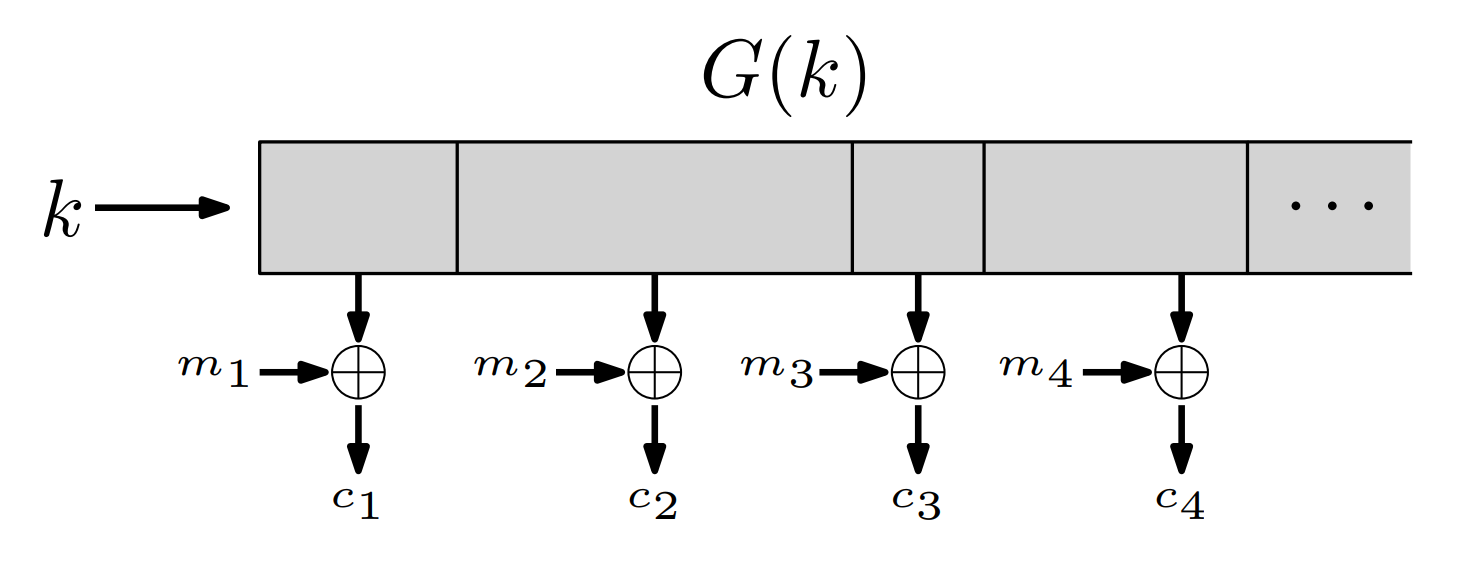
\includegraphics[width=0.5\textwidth]{images/synchronized_mode}
    \caption{Synchronized mode: Stream cipher with internal state (stateful).}
\end{figure}
\begin{figure}[h]
    \centering
    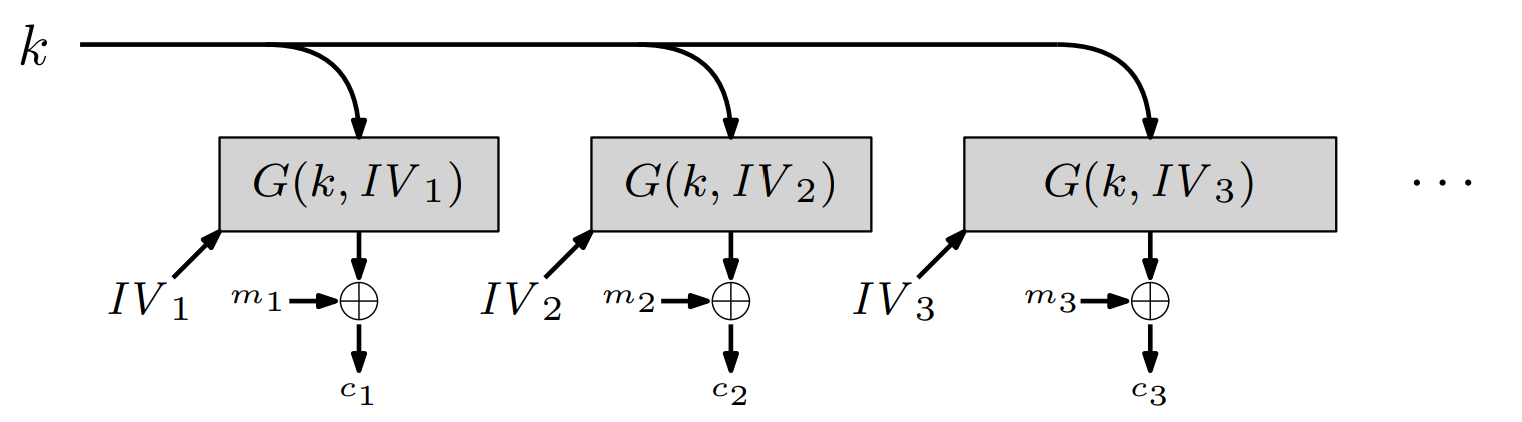
\includegraphics[width=0.5\textwidth]{images/unsynchronized_mode}
    \caption{Unsynchronized mode: Stream cipher without internal state (stateless).}
\end{figure}
\end{document}